\section{Filesystems}
Filesystems are used to store data on for instance a hard drive of a computer in the cloud. Google Drive is a filesystem that enables users to save their data online up to 15 GB for free\cite{CloudStorageWork} using their clusters of distributed storage devices, meaning that the data is saved on their servers which can be located wherever\cite{DistributedStorageWhat}. Paying customers can achieve a higher amount of storage using the service.

A Unix filesystem uses a data structure called an \textit{inode}. An inode keeps track of the metadata for the files in the filesystem, and a directory simply contains the file names and each file or directory's inode id. Using a lookup, the system can then learn about the file - for instance where it is located and how big it is as can be seen in Figure~\ref{fig:inode_diag} % FIXME: CITATION NEEDED 
Each inode entry can contain any number of metadata information that might be relevant for the system, such as creation time and last updated.

\begin{figure}[!ht]
	\begin{center}
	  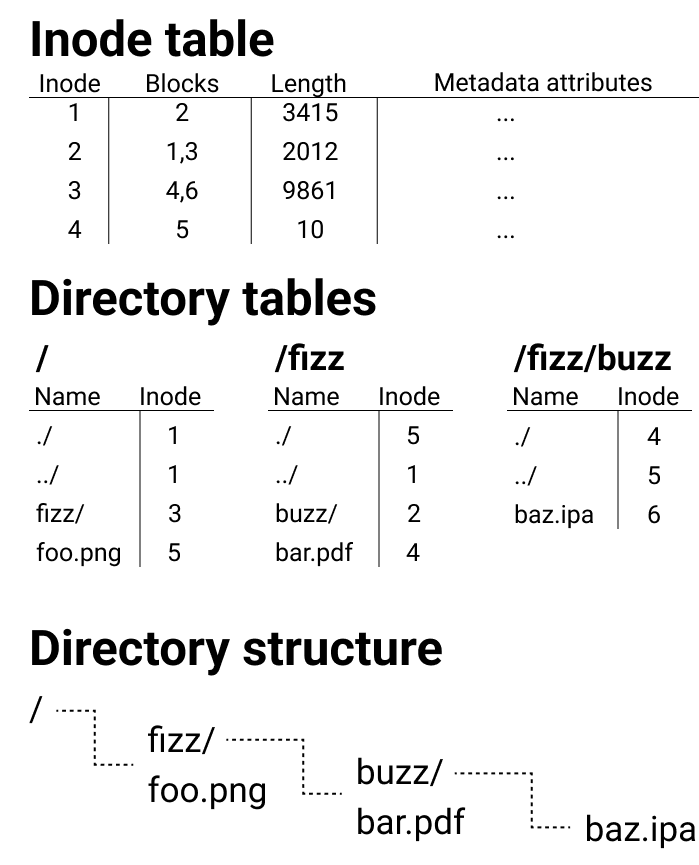
\includegraphics[width=0.8\textwidth]{figures/inode_diagram.png}
	\end{center}
	\caption{Basic structure of inode based filesystem}
	\label{fig:inode_diag}
\end{figure}

Looking at the 4 main file systems of windows, they all have many, sometimes different, functionalities such as links and named streams as well limitations such as a defined theoretical maximum file size\cite{mikbenFileSystemFunctionality}. This is set to 16 exbibytes for NTFS, exFAT, and UDF, and for FAT32 it is set to 4 gigabytes. 

\subsection{Image structures}
Different file types has different protocols and definitions of how they should be encoded and decoded, for instance a JPEG and a PNG can display similar content but the data they store is different. At the lowest level all files consists of a string of binary digits no matter the file type. If one would represent an arbitrary file of $X$ bytes, each byte (0x00 - 0xFF) can be represented as a character such as the ASCII keyset and we can therefore represent this file as $X$ different characters. Using the same set of characters for encoding and decoding we can get a symmetric relation for representing a file as a string of characters. 

This string of $X$ bytes can also be used as the data in an image. An image can be abstracted as a $h * w$ matrix, where each element is a pixel. Each pixel represents a color which can be represented as a number. One can therefore imagine that we can use this string of $X$ bytes to assign colors in this color matrix by assigning the first $Y$ bytes as the first pixels color, the next $Y$ bytes as the following pixels color and so forth. The value of $Y$ depends on the color type and depth of the image, for simplicity we can imagine an 8-bit RGB value, i.e. $Y$ is 3 bytes (1 byte per Red, Green and Blue). This means that $X$ bytes of data can be represented as 
$$ceil(\frac{X}{3})$$ 
pixels, where $ceil$ rounds a float to the closest larger integer. For a file of 1Mb, i.e. $X = 1'000'000$ we need $333'334$ pixels. The values of $h$ and $w$ are arbitrary but if we for instance want a square image we can set $ h = w = 578$ which means that there will be $334'084$ pixels in total, and the remaining $750$ pixels will just be fillers to make the image a reasonable size. We could however choose $h = 1$ and $w = 333'334$ which would mean a very wide image but would not require filler pixels.